\documentclass[12pt,a4paper,fleqn]{article}
\title{Progress Report}
\author{Syed Ahmad Raza}
\date{2017.12.27}
\usepackage{mathtools}
\usepackage{graphicx}
\usepackage{color}          % for color eps output
% \usepackage{afterpage}
\usepackage{float}          % to force a figure placement with [H] command
\usepackage{enumitem}
\usepackage{newtxtext}
\usepackage{newtxmath}
%\usepackage{layouts}       % for: \printinunitsof{in}\prntlen{\textwidth}

\begin{document}
\maketitle
\tableofcontents
\pagebreak

\section{Solution of Navier-Stokes equations using Finite Volume Method for unequal grid intervals}

Continuity equation is
\begin{equation}\label{eq:continuity}
\nabla \cdot \mathbf{u} = 0 \quad,
\end{equation}
and Navier-Stokes equation is
\begin{equation}\label{eq:navier-stokes}
\frac{\partial \mathbf{u}}{\partial t}+\nabla \cdot (\mathbf{u}\mathbf{u}) = -\frac{1}{\rho}\nabla p + \nu \nabla^2 \mathbf{u}+\mathbf{f} \quad.
\end{equation}
where $\mathbf{u}$ is the velocity vector, \textit{p} is the pressure, $\rho$ is density of the fluid, and $\mathbf{f}$ is body force per unit mass.

Ignoring the body force $\mathbf{f}$, we are left with
\begin{equation}\label{eq:navier-stokes-no-f}
\frac {\partial \mathbf{u}}{\partial t} = -\frac{1}{\rho}\nabla p -\nabla \cdot (\mathbf{uu}) + \nu \nabla^2 \mathbf{u} \quad.
\end{equation}

\subsection{Projection method}
Using a new vector $\mathbf{u}^*$ for intermediate velocity and \textit{n} as the index for time step, projection method is used to decompose Navier-Stokes equation in \eqref{eq:navier-stokes-no-f} into two parts,
\begin{equation}\label{eq:projection01}
\frac{\mathbf{u}^*-\mathbf{u}^n}{\Delta t} = -\nabla \cdot (\mathbf{u}\mathbf{u})+ \nu \nabla^2 \mathbf{u} \quad,
\end{equation}
which accounts for the convective and diffusive terms, and
\begin{equation}\label{eq:projection02}
\frac{\mathbf{u}^{n+1}-\mathbf{u}^*}{\Delta t}=-\frac{1}{\rho}\nabla p \quad,
\end{equation}
which accounts for the pressure term.

\subsection{Discretization of the convective and diffusive terms}
The convective and diffusive terms from equation \eqref{eq:projection01} can be discretized using the individual components. For the $u$-component, equation \eqref{eq:projection01} can be written as
\begin{equation} \label{eq:convective-diffusive-u}
\frac{\partial u}{\partial t} = -\frac{\partial uu}{\partial x} -\frac{\partial uv}{\partial y} + \nu\left[\frac{\partial^2u}{\partial x^2} + \frac{\partial^2u}{\partial y^2}\right] \quad,
\end{equation}
which can be discretized as
\begin{align}\label{eq:discretized_convective-diffusive-u}
\frac{\partial u}{\partial t} =
{}& - \frac{u_e^2 - u_w^2}{Dx} - \frac{u_n v_n - u_s v_s}{Dy} + \nu\left[
\left\{
\frac{u_{i+1,j}-u_{i,j}}{Dx1}
- \frac{u_{i,j}-u_{i-1,j}}{Dx2}
\right\}
\frac{1}{Dx}
\right.\nonumber\\
& \left. + \left\{
\frac{u_{i,j+1}-u_{i,j}}{Dy}
- \frac{u_{i,j}-u_{i,j-1}}{Dy3}
\right\}
\frac{1}{Dy2}
\right] \quad ,
\end{align}
where, for the \emph{diffusion terms}, second-order central scheme has been used. Similarly for the $v$-component, equation \eqref{eq:projection01} will be
\begin{equation} \label{eq:convective-diffusive-v}
\frac{\partial v}{\partial t} = -\frac{\partial uv}{\partial x} -\frac{\partial vv}{\partial y} + \nu\left[\frac{\partial^2v}{\partial x^2} + \frac{\partial^2v}{\partial y^2}\right] \quad ,
\end{equation}
which can be and discretized as
\begin{align}\label{eq:discretized_convective-diffusive-v}
\frac{\partial v}{\partial t} =
{}& - \frac{u_e v_e - u_w v_w}{Dx} - \frac{v_n^2 - v_s^2}{Dy} \nonumber\\
& + \nu\left[
\left\{
\frac{v_{i+1,j}-v_{i,j}}{Dx}
- \frac{v_{i,j}-v_{i-1,j}}{Dx3}
\right\}
\frac{1}{Dx2}
\right.\nonumber\\
& \left. + \left\{
\frac{v_{i,j+1}-v_{i,j}}{Dy1}
- \frac{v_{i,j}-v_{i,j-1}}{Dy2}
\right\}
\frac{1}{Dy}
\right] \quad .
\end{align}

\begin{figure}[H]
    \centering
    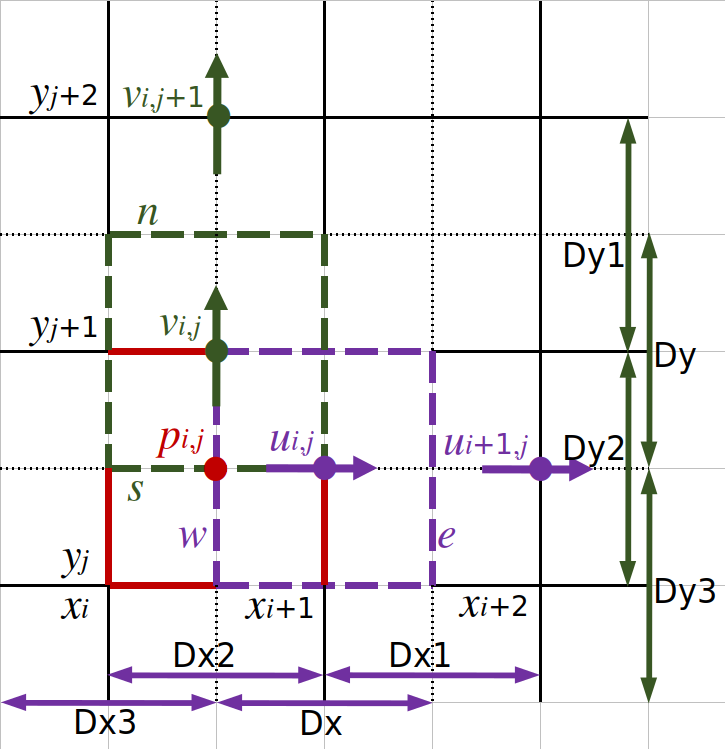
\includegraphics[width=0.5\textwidth]{staggered_grid.png}
    \caption{Visual representation of the staggered grid used for discretization in Finite Volume Method}
    \label{fig:staggered-grid}
\end{figure}

\subsubsection{Substitutions for velocities in the convective terms}
Following formulas are used for the velocities $u_n, u_s, v_e$ and $v_w$,
\begin{equation*}
\begin{aligned}
u_n &= u_{i,j} + \frac{u_{i,j+1} - u_{i,j}}{Dy}\\
u_s &= u_{i,j} - \frac{u_{i,j} - u_{i,j-1}}{Dy3}
\end{aligned}
\qquad\qquad
\begin{aligned}
v_e &= v_{i,j} + \frac{v_{i+1,j} - v_{i,j}}{Dx}\\
v_w &= v_{i,j} - \frac{v_{i,j} - v_{i-1,j}}{Dx3}
\end{aligned}
\end{equation*}

For rest of the velocities in the convective terms, namely $u_e, u_w, v_n$ and $v_s$, the upwind scheme was used.

\paragraph{Upwind scheme}\mbox{}\\
For positive velocities,
\begin{equation*}
\begin{aligned}
u_e = u_{i,j}\\
u_w = u_{i-1,j}
\end{aligned}
\qquad\qquad
\begin{aligned}
v_n = v_{i,j}\\
v_s = v_{i,j-1}
\end{aligned}
\end{equation*}
For negative velocities,
\begin{equation*}
\begin{aligned}
u_e = u_{i+1,j}\\
u_w = u_{i,j}
\end{aligned}
\qquad\qquad
\begin{aligned}
v_n = v_{i,j+1}\\
v_s = v_{i,j}
\end{aligned}
\end{equation*}

\subsubsection{Adams-Bashforth scheme}
Euler scheme was utilized for the first time step and Adam-Bashforth scheme was used for the remaining. Denoting the terms on the right-hand side of equation \eqref{eq:projection01} with $\mathcal{F}(\mathbf{u})$, the second order Adams-Bashforth scheme can be applied using
\begin{equation}\label{eq:adams-bashforth}
\frac{\mathbf{u}^*-\mathbf{u}^n}{\Delta t} = \frac{3}{2}\mathcal{F}(\mathbf{u}^n)-\frac{1}{2}\mathcal{F}(\mathbf{u}^{n-1})\quad .
\end{equation}

\subsection{Poisson equation of pressure}
Using the conservation of mass principle for the $n+1^{\text{st}}$ time step,
\begin{equation} \label{eq:continuity-n+1}
\nabla \cdot \mathbf{u}^{n+1} = 0 \quad ,
\end{equation}
and substituting equation \eqref{eq:projection02}, we get the Poisson equation for pressure
\begin{equation} \label{eq:poisson}
\nabla^2 p^{n+1} = \frac{\rho}{\Delta t}\nabla \cdot \mathbf{u}^* \quad ,
\end{equation}
which can be written as
\begin{equation} \label{eq:poisson-components}
\frac{\partial^2 p}{\partial x^2} + \frac{\partial^2 p}{\partial y^2}
= \frac{1}{\Delta t} \left(\frac{\partial u^*}{\partial x} + \frac{\partial v^*}{\partial y}\right) \quad .
\end{equation}
Integrating it twice, discretizing and rearranging leads to
\begin{align}
p_{i,j}^{n+1} =
&\frac{1}{\left[ - \frac{Dy}{Dx1} - \frac{Dy}{Dx2} - \frac{Dx}{Dy1} - \frac{Dx}{Dy2} \right]}
\nonumber \\
&\times
\left[
- \frac{Dy}{Dx1}p_{i+1,j} - \frac{Dy}{Dx2}p_{i-1,j} - \frac{Dx}{Dy1}p_{i,j+1} - \frac{Dx}{Dy2}p_{i,j-1}
\right. \nonumber \\
&\left.
+ \frac{1}{\Delta t}\left\{
\left(u^*_{i,j}-u^*_{i-1,j}\right) \Delta y
+ \left(v^*_{i,j}-v^*_{i,j-1}\right) \Delta x
\right\}
\right]
\quad .
\end{align}
Using successive over-relaxation method (SOR),
\begin{align}
p_{i,j}^{n+1} =& \left(1 - \omega\right)p_{i,j} + \omega
\Bigg[
\frac{1}{\left( - \frac{Dy}{Dx1} - \frac{Dy}{Dx2} - \frac{Dx}{Dy1} - \frac{Dx}{Dy2} \right)}
\nonumber \\
&\times
\left\{
- \frac{Dy}{Dx1}p_{i+1,j} - \frac{Dy}{Dx2}p_{i-1,j} - \frac{Dx}{Dy1}p_{i,j+1} - \frac{Dx}{Dy2}p_{i,j-1}
\right. \nonumber \\
&\left.
+ \frac{1}{\Delta t}\left(
\big(u^*_{i,j}-u^*_{i-1,j}\big) \Delta y
+ \big(v^*_{i,j}-v^*_{i,j-1}\big) \Delta x
\right)
\right\}
\Bigg]
\quad ,
\end{align}
where the relaxation factor, $\omega = 1.8$.
Finally, the correct velocity can be found using
\begin{equation}
\mathbf{u}^{n+1} = \mathbf{u}^* - \frac{\Delta t}{\rho}\cdot \nabla p^{n+1} \quad ,
\end{equation}
which is, for $u$- and $v$-components,
\begin{equation}
u^{n+1}_{i,j} = u^*_{i,j} - \frac{\Delta t}{\rho}\cdot \frac{p_{i+1,j}^{n+1} - p_{i,j}^{n+1}}{\Delta x}
\end{equation}
and
\begin{equation}
v^{n+1}_{i,j} = v^*_{i,j} - \frac{\Delta t}{\rho}\cdot \frac{p_{i,j+1}^{n+1} - p_{i,j}^{n+1}}{\Delta y}
\end{equation}

\subsection{Future work}
\begin{itemize}
\item Solve energy equation for heat transfer
\item Solve for 3D domain
\end{itemize}

\end{document}
